
\newpage

\section*{Computing a $\rho$-ordering}
In the previous section, we defined valuative capacity for a compact subset $S$ of an ultrametric space $(M, \rho)$. We also got a glimpse into the way the valuative capacity of $S$ interacts with its other properties, such as the set of distances occurring in $S$ and the lattice of closed balls in $S$ (or equivalently, if $S$ has enough structure, the lattice of subgroups).\\

In this section, we offer a more detailed study of the interaction between the valuative capacity of $S$ and the lattice of closed balls in $S$. In particular, we  show how, in all cases (with $S$ compact), the latter can be used to compute the first $n$ terms of a $\rho-$ordering of $S$ (for any $n < \infty$) and how, in some cases, this extends to being able to compute the valuative capacity of $S$.\\

We begin by letting $S$ be, as before,  a compact subset of an ultrametric space $(M, \rho)$, and by letting $\Gamma_S =\{\gamma_0, \gamma_1,\ldots,\gamma_\infty=0\}$ be the set of distances in $S$.  Now fix some $k \in \mathbb{N}$, and consider for a moment the set of closed balls of radius $\gamma_k$ in $S$. We could denote these alternatively by $B^M(x, \gamma_k) \cap S$ or by  $B^S(x, \gamma_k)$, but when there is no risk of confusion, we will denote them simply by $B(x, \gamma_k)$. Clearly, the set  $\{B(x, \gamma_k); x \in S\}$ forms a cover of $S$ and since $S$ is compact, we must have some $x_1,\ldots, x_n$  such that $S= \cup_{i=1}^n B(x_i, \gamma_k)$. In fact,  since $\rho$ is an ultrametric, we can pick the $x_i$'s so that $\cup_{i=1}^n B(x_i, \gamma_k)$ will be a disjoint union and therefore a partition of $S$. Note that both $n$ and the $x_i$'s depend on our fixed $k$, but that $n$ is independent of the $x_i$'s, since any choice of centres is equivalent. We rephrase this with following definition and lemma:

\begin{definition*}
For $S$ and $\Gamma_S$ as above, and $k \in \mathbb{N}$, fixed,  define $\sim_k$ to  be the relation on $S$ given by \[x \sim_k y\text{ if and only if  }\rho(x,y) \leq \gamma_k\] i.e.,  $x \sim_k y$ if and only if $B_{\gamma_k}(x) = B_{\gamma_k}(y)$.
\end{definition*}

The fact $\sim_k$ is an equivalence relation on $S$ is equivalent to the observation that every point in a ultrametric ball is at its centre:

\begin{lemma*}
Let  $S$ and $\Gamma_S$ be as above, then $\sim_k$ is an equivalence relation on $S$.
\end{lemma*}

\begin{proof}
$\sim_k$ is clearly reflexive and symmetric, since $\rho$ is a metric. Transitivity results from the ultrametric property of $\rho$: if $x \sim_k y$ and $y \sim_k z$, then $$\rho(x, z) \leq \max(\rho(x,y), \rho(z,y)) \leq \gamma_k$$ so $x \sim_k z$. 
\end{proof}

 We denote the set of equivalence classes of $S/\sim_k$ by $S_{\gamma_k}$. We have defined  $S_{\gamma_k}$ to be the set of equivalence classes in $S$ under the relation $\sim_k$, which is equivalent to letting $S_{\gamma_k}$ be the set of closed balls of fixed radius $\gamma_k$ in  $S$. We now offer a third perspective on the elements on $S_{\gamma_k}$, which is due to \cite{na},

\begin{lemma*}
For each $k$, the elements of $S_{\gamma_k}$, that is, the closed balls of radius $\gamma_k$, themselves form an ultrametric space, where the metric is given by:
\[ \rho_k(B(x, \gamma_k),B(y, \gamma_k)) = 
\begin{cases}
\rho(x,y), & \text{if } \rho(x,y) > \gamma_k \\
0, & \text{if }   \rho(x,y) \leq \gamma_k \text{, i.e., } B(x, \gamma_k)=B(y, \gamma_k)
\end{cases}
\]
\end{lemma*}

\begin{proof}
$\rho_k$ is reflexive, symmetric and transitive since $\rho$ is. Likewise, $\rho_k$ satisfies the ultrametric property, since $\rho$ does: let $B(x, \gamma_k),B(y, \gamma_k)$ and $B(z, \gamma_k)$ be any three elements of $S_{\gamma_k}$ and suppose $\rho_k(B(x, \gamma_k),B(y, \gamma_k)) > 0 $. Then,
\begin{align*}
\gamma_k < \rho_k(B(x, \gamma_k),B(y, \gamma_k)) && \\
= \rho(x,y) \leq \max(\rho(x,z), \rho(y,z)) && \\
= \max(\rho_k(B(x, \gamma_k), B(z, \gamma_k)), \rho_k(B(y, \gamma_k),B(z,\gamma_k)))
\end{align*}
since $ \gamma_k < \max(\rho(x,z), \rho(y,z))$ implies that at least one of $\rho_k(B(x, \gamma_k), B(z, \gamma_k))$ or $\rho_k(B(y, \gamma_k),B(z,\gamma_k))$ is greater than $0$.
\end{proof}

So now the elements of $S_{\gamma_k}$ may be viewed as either equivalence classes, closed balls of fixed radius, or points in a new metric space. We  make a final definition and introduce some notation before moving on.

\begin{definition*}
Let $S$ and $\Gamma_S$ be as above. Define $\beta(i)_{i=0}^{\infty}$ to be the sequence given by $\beta(i) = \lvert  S_{\gamma_i}\rvert$, which is an invariant of $S$ and which counts the number of connected components of $S_{\gamma_i}$ when viewed as a metric space. When necessary, we use $\beta^S(i)$ to denote the $\beta$ sequence for a given, compact  ultrametric space $S$. Adapting the terminology in \cite{fp}, we call $\beta^S(i)$ the \textbf{structure sequence} of $S$.
\end{definition*}

\begin{notation*}
Let $S_{\gamma_k}$ be as above. We denote the elements of $S_{\gamma_k}$ by $B^k_1, \ldots, B^k_{\beta(k)}$ or by $B^{S,k}_1, \ldots, B^{S,k}_{\beta(k)}$, when necessary.
\end{notation*}


We return to the sequence $\beta(i)$ at the end of this section. For now, we show how a $\rho-$ordering of $S$ can be built recursively from the spaces $S_{\gamma_k}$. This begins by noting that the spaces themselves can be built recursively:

\begin{observation*}
Let $S$, $\Gamma_S$, and $S_{\gamma_k}$ be as above. Then $S_{\gamma_k+1}$ can be constructed by partitioning each of the closed balls in $S_{\gamma_k}$ into closed balls of radius $\gamma_{k+1}$ and taking their union:  Let $B(x_i, \gamma_k)$  be an element of $S_{\gamma_k}$, denoted by  $B^k_i$. Then, there exists $x_{i,1},\ldots, x_{i,l_{i}} \in B^k_i$ such that,

\[B^k_i=  \cup_{j=1}^{l_i} B(x_{i,j}, \gamma_{k+1})\] 

and so

\[S_{\gamma_{k+1}} =  \cup_{i=1}^{\beta(k)}   \cup_{j=1}^{l_i} B(x_{i,j}, \gamma_{k+1}) = \cup^{\beta(k+1)}_{j=1}B^{k+1}_{j}\] 


where $\cup_{j=1}^{l_i} B(x_{i,j},\gamma_{k})=B(x_i, \gamma_{k+1}) = B^k_i$, $\forall i$.
\end{observation*}

We can represent this schematically as below:

\tikzset{font=\small,
level distance=1.75cm,
}

\begin{center}
\begin{tikzpicture}
\Tree [.  $B^0_1$ \edge;
          [. $B^k_1$   [. $B^{k+1}_1$ ]
		       [. $B^{k+1}_2$ ]
		        [. $\ldots$ ]
                              [. $B^{k+1}_{l_1}$ ] ] \edge;
          [.$B^k_2$ [. $B^{k+1}_{l_1 + 1}$ ]
		       [. $B^{k+1}_{l_1 + 2}$ ]
	                  [. $\ldots$ ]
                             [. $B^{k+1}_{l_1 + l_2}$ ] ] \edge;
          [.$\ldots$ ]  \edge;
          [.$B^k_{\beta(k)}$ [. $B^{k+1}_{\sum\limits_{\mathclap{i < \beta(k)}}  l_i + 1 }$ ]
			                   [. $\ldots$ ]
                                                    [. $B^{k+1}_{\beta(k+1)}$ ] ] ]
\end{tikzpicture}
\end{center}

\begin{notation*}
If $S$ is a compact subset of an ultrametric space, the lattice of closed balls in $S$, as depicted above, is denoted by $T_s$.\\
\end{notation*}

We make a few observation on the relationships between the vertices in $T_s$. First we consider the distance between two vertices in $T_s$. Since each vertex represents a ball in an ultrametric space, it is well-defined to let the distance between vertices be equal to the distance between a choice of centres for those balls. This is equal to the diameter of the smallest closed ball that contains any two vertices, that is, the level of their join. In particular, for any $k$ and any $i < \beta(k)$, the distances between the children of $B^k_i$ will be $\gamma_k$ and for any $i \neq j$ the distance between the children of $B^k_i$ and $B^k_j$ will be equal to the distance between  $B^k_i$ and $B^k_j$ (which will be some $\gamma_{m}, m <k$).\\

Finally, note that without loss of genearlity, for any $k \in \mathbb{N}$, we can reindex the $B^k_i$'s so that they give the first $\beta(k)$ terms of a $\rho_k$-ordering of $S_{\gamma_k}$, when the latter is viewed as a (finite) metric space. If the $B^k_i$'s are so indexed, then finding a $\rho_{k+1}$-ordering of $S_{\gamma_{k+1}}$ is straightforward: select a $B^{k+1}_j$ from each of the $B^k_i$'s in order and then start over.  The following two propositions show how this can be used to recursively build a $\rho-$ordering of $S$.

\begin{proposition*} 
Let be $S$ a compact subset of an ultrametric space $(M, \rho)$ and $\Gamma_S$, the set of distances in $S$. If $S_{\gamma_k}$ is a partition of $S$ as described above for $\gamma_k \in \Gamma_S$ with $k < \infty$, where the elements are indexed according to a $\rho_k$-ordering of $S_{\gamma_k}$, then the first $\beta(k+1)$ terms in a $\rho_{k+1}$-ordering of $S_{\gamma_{k+1}}$ can be found by selecting at each stage $n$, a child from $B^k_\overline{n}$, where $\overline{n} = n \mod \beta(k) +r $ and $r$ is minimal in $\{0,\ldots,\beta(k)-1\}$ such that $B^k_{n \mod \beta(k) +r}$ still has unused children.

\begin{proof}
Let $S$, $S_{\gamma_K}$, and $S_{\gamma_{k+1}}$ be as above. In particular, suppose the elements of $S_{\gamma_k}$ are indexed according to a $\rho_k-$ordering. Denote the elements of $S_{\gamma_{k+1}}$ by $B^{k+1}_{i,j}$ where the first subscript indicates that the elements is a child of $B^k_i$. To form a $\rho_{k+1}$ ordering of $S_{\gamma_{k+1}}$, we must maximize the product of distances at each step $n$.\\

Now note that $\Gamma_{S_{\gamma_k}} = \{\gamma_0, \gamma_1,\ldots, \gamma_{k-1}\}$ and $\Gamma_{S_{\gamma_{k+1}}} = \{\gamma_0, \gamma_1,\ldots, \gamma_{k-1}, \gamma_{k}\}$. That is, the distances in $S_{\gamma_{k+1}}$ are the same as the distances in $S_{\gamma_k}$, although they also include the smaller distance $\gamma_k$. Since we know that the elements $B^k_1,\ldots,B^k_{\beta(k)}$ already maximizes the product of distances in $\{\gamma_0, \gamma_1,\ldots, \gamma_{k-1}\}$, the first $\beta(k)$ terms of a $\rho_{k+1}$-ordering of $S_{k+1}$ can be found by taking $B^k_{1,j_1},\ldots, B^k_{1,j_{\beta(k)}}$ for any choice of $j$'s. At this point, any choice of next element will produce a copy of $\gamma_k$ in the $\rho_{k+1}$-sequence; however, if we chose another child of $B^k_{1}$, we are able to keep building the ordering in a canonical fashion, since we know that we will then be able to maximize the product at the next step by chosing another child of $B^k_{2}$.\\

We see then that a $\rho_{k+1}$-ordering of $S_{\gamma_{k+1}}$ is found by minimizing the number of times $\gamma_k$ is introduced into the $\rho_{k+1}$-sequence and maximizing the product among the $\gamma_0, \gamma_1,\ldots, \gamma_{k-1}$, and the latter is already known to be achieved by taking the $B^k_i$ in order.  If the $B^k_i$'s all have the same number of children, then we can always select a child of $B^k_\overline{n}$, where $\overline{n} = n \mod \beta(K)$ at each stage $n$, $n < \beta(k+1)$, since there will always be one available. On the other hand, suppose the $B^k_i$ have an unequal number of children and $n$ is the first step at which all the children of $B^k_{\overline{n}}$ have been exhausted. What element will maximize the $\rho_{k+1}-$sequence?\\

Consider the space $(S_{\gamma_k} \setminus B^k_{\overline{n}})$. Removal of $B^k_{\overline{n}$ will not effect the first $m$ terms of a $\rho_k$-ordering of this space, for $m < \overline{n}$, since if a sequence of elements maximizes a function over a set $X$, they will also maximize that function of a subset of $X$ (provided they themselves remain in the subset). Then the $\rho_k-$sequence of $(S_{\gamma_k} \setminus B^k_{\overline{n}})$ begins $\{B^k_1,\ldots, B^k_{\overline{n}-1}\}$.\\

Moreover, if $B^k_{\overline{n}+1}$ maximizes $\prod^{\overline{n}}_{i=1} \rho_{k}(x, B^k_i)$ over $S_{\gamma_k}$, then it also maximizes $\prod^{\overline{n}-1}_{i=1} \rho_{k}(x, B^k_i)$ over $(S_{\gamma_k} \setminus B^k_{\overline{n}})$, since $\prod^{\overline{n}}_{i=1} \rho_{k}(x, B^k_i) = (\prod^{\overline{n}-1}_{i=1} \rho_{k}(x, B^k_i)) \cdot \rho_{k}(x, B^k_{\overline{n}})$.\\

Then the $\rho_k-$sequence of  $(S_{\gamma_k}\setminus B^k_{\overline{n}})$ is simply $\{B^k_1,\ldots, B^k_{\overline{n}-1}, B^k_{\overline{n}+1},\ldots, B^k_{\beta(k)}\}$.\\

Now we see that $\rho_{k+1}-$sequence of $S_{\gamma_{k+1}}$ is maximized by simply skipping over $B^k_{\overline{n}}$, should all its children be exhausted, and selecting a child from $B^k_{\overline{n}+1}$. Then a $\rho_{k+1}-$ordering of $S_{\gamma_{k+1}}$ is found by selecting elements of each $B^k_i$ in order as much as possible, and skipping to $B^k_{i+1}$, when it is not possible.

\end{proof}

The above results quickly leds to a recursive contruction for a $\rho-$ordering of $S$.

\begin{proposition*}
Let be $S$ a compact subset of an ultrametric space $(M, \rho)$ and let $\Gamma_S$ be the set of distances in $S$. Let $S_{\gamma_k}$ is a partition of $S$ as described above for $\gamma_k \in \Gamma_S$ with $k < \infty$, where the elements are indexed according to a $\rho_k$-ordering of $S_{\gamma_k}$. Let $x_{i,j}$ denote a choice of centre for the element $B^{k+1}_{i,j}$. Then the first $\beta(k+1)$ elements of a $\rho-$ordering of $S$ can be found by forming a matrix, $A_k$, whose $(i,j)^{th}$-entry is $x_{i,j}$, as shown below, and then concatenating the rows (where the columns are padded by * if necessary).
\end{proposition*}

\[A_k=
 \begin{pmatrix}
  x_{1,1} & x_{2,1} & \ldots  &x_{n,1} \\
  x_{1,2} & x_{2,2} &\ldots &x_{n,2} \\
  \vdots & \vdots & \ddots & \vdots \\
  x_{1,l_1} & x_{2,l_2} & \ldots &x_{n,l_n}
 \end{pmatrix}
\]


\begin{proof}
Note that the entries in each column are points in the ball $B_{\gamma_k}(x_i)$ so that the pairwise distance between columns is constant and always exceeds the distance between elements within a column. Moreover, the columns are organized such that for any $j$, $x_{n,j}$ maximizes$\prod_{i=1}^{n-1} \rho_(x_{n,j},x_{i,j})$ since $\prod_{i=1}^{n-1} \rho_(x_{n,j},x_{i,j}) = \prod_{i=1}^{n-1} \rho_(x_{n,1},x_{i,1}) = \prod_{i=1}^{n-1} \rho_(x_{n},x_{i})$ and the $x_i$'s are indexed according a $\rho_k$-ordering of $S_{\gamma_k}$.

Then a $\rho_{\gamma_{k+1}}$-ordering of $S_{\gamma_{k+1}}$ is obtained by minimizing the number of elements from any one column and by taking the points $x_{i,j}$ (for fixed $j$) in sequence. For example, by concatenating the rows.
\end{proof}

Note that in building the $\rho_{k+1}-$ordering of $S_{\gamma_{k+1}}$, we imposed an ordering on the elements of $S_{\gamma_k}$, but not on the individual children of a given $B^k_i$. Any choice of indexing on these children is equivalent since the distances between any two of them is $\gamma_k$ and the distance between any one of them and a child of some $B^k_j$, $i \neq j$, is the same, since each $B^k_i$ is a ball in an ultrametric space. For this reason, it also did not depend which child was chosen at a given stage. Suppose then that we have created $T_s$ and (arbitrarily) indexed the children of each vertex. Then, there is no loss of genearlity in assuming that at each stage, we select a child with smallest index among its siblings, that is, that we select the leftmost available child in $T_s$. Since for ease of indexing, we will often assume a $\rho-$ordering has been built by this convention, we introduce the following definition.

\begin{definition*}
The $\rho-$ordering of $S$ formed by pulling elements from left to right in (a choice of) $T_s$ is call the \textbf{canonical $\rho$-ordering} of $S$ (with respect to $T_s$).
\end{definition*}

\begin{example}
$\mathbb{Z}$ with any prime
\end{example}

\begin{example}
$\mathbb{Z} \setminus 4\mathbb{Z} \subset (\mathbb{Z}, \lvert \cdot \rvert_2)$
\end{example}


\begin{corollary*}
Interweaving the bottom row of the lattice of closed balls for a set $S$ gives a $\rho$-ordering of $S$. 
\end{corollary*}


\begin{lemma*}
If $\delta$ denotes the $\rho$-ordering of $S$ formed by pulling from left to right in $T_s$, then \[\rho(\delta(n),\delta(m))=\gamma_k\] if and only if \[ n=m \mod \beta(k) \text{  and } n \neq m \mod \beta(k+1)\]
\end{lemma*}

\begin{lemma*}
$\lfloor\frac{n}{q} \rfloor$ counts the numbers strictly less than $n$ that are congruent to $n \mod q$.
\end{lemma*}

\begin{proof}
Every multiple of $q$ produces exactly one of the numbers from $1$ to $q$ and exactly one of those is the residue class of $n$ modulo $q$. The remainder is the residue class of $n$ itself and since we only want the numbers strictly less than $n$, we ignore this by taking the floor.
\end{proof}


\begin{proposition*}
\[v_{\gamma_k}(\sigma(n)) = \lfloor\frac{n}{\beta(k)}\rfloor - \lfloor\frac{n}{\beta(k+1)}\rfloor \]
\end{proposition*}

\begin{definition*}
Let $S$ be as above. We say that $S$ is \textbf{semi-regular} if $T_{B^k_i} = T_{B^k_j}$, $\forall k \in \mathbb{N}$ and  $i,j \in \beta(k)$. That is, $S$ is semi-regular if each ball of radius $\gamma_k$ breaks into the same number of balls of radius $\gamma_{k+1}$, for all $k$. If there exists an $n \in \mathbb{N}$ such that $T_{B^n_i} = T_{B^n_j}$, i.e.  each ball of radius $\gamma_N$ breaks into the same number of balls of radius $\gamma_{N+1}$, for all $N \geq n$, then we say $S$ is \textbf{eventually semi-regular}.
\end{definition*}
cite Amice or Fares or both here.

\begin{corollary*}
If $S$ is a semi-regular ultrametric space, $\Gamma_S$ is the sequence of distances in $S$, and $\beta$ is the structure sequence of $S$, then \[v_{\gamma_k}(\sigma(n)) = \lfloor\frac{n +\beta(k)}{\beta(k+1)}\rfloor \]
\end{corollary*}

\begin{example}
Consider the ultrametric space $(\mathbb{Z}, \rvert \cdot \lvert_p)$  for any prime $p$. The corollary gives 
\[v_{1}(\sigma(n)) = \lceil\frac{n}{p}\rceil\]
\[v_{\frac{1}{p}}(\sigma(n)) = \lceil\frac{n +p }{p^2}\rceil\]
\[v_{\frac{1}{p^2}}(\sigma(n)) = \lceil\frac{n + p^2}{p^3}\rceil\]
\[v_{\frac{1}{p^3}}(\sigma(n)) = \lceil\frac{n + p^3}{p^4}\rceil\]

So that \[\sigma(n) = (\frac{1}{p})^ { \lceil\frac{n + p}{p^2}\rceil + 2 \cdot  \lceil\frac{n +p^2}{p^3}\rceil + 3 \cdot  \lceil\frac{n + p^3}{p^4}\rceil + \ldots}\]
\[ = (\frac{1}{p})^ { \sum_{i=1}^\infty i \cdot \lceil\frac{n + p^i}{p^{i+1}}\rceil }\]
\[ = (\frac{1}{p})^ { \sum_{i=1}^\infty i \cdot \lceil\frac{pn}{p^{i+1}}\rceil -  \lceil\frac{n}{p^{i+1}}\rceil }\]
\[ = (\frac{1}{p})^ { \sum_{i=1}^\infty i \cdot \lceil\frac{n}{p^{i}}\rceil -  \lceil\frac{n}{p^{i+1}}\rceil }\]
\[ = (\frac{1}{p})^ { \sum_{i=1}^\infty \lceil \frac{n}{p^{i}}\rceil}\]
\end{example}

\begin{corollary*}
If $S$ is a (eventually) semi-regular ultrametric space and the $\alpha$ sequence of $S$ is (eventually)  periodic, then the valuative capacity of $S$ is algebraic.
\end{corollary*}

%\begin{corollary*}
%Suppose $S$ and $T$ are compact subsets of an ultrametric space $M$ with $\Gamma_S = \Gamma_T$ and $\mid S_{\gamma_k}\mid =\mid T_{\gamma_k}\mid$, $\forall k$. Then $\omega(S) = \omega(T)$. 
%\end{corollary*}
%\begin{itemize}
%\item i think this coincides with translation invariance when there is a group operation
%\end{itemize}

%\begin{notation*}
%If $S$ is (eventually) semi-regular, then the structure sequence of $B^1_1$ (respectively, $B^N_1$) is also an invariant of $S$, which we denote by $\alpha^S(i)$.\\
%\end{notation*}

Semi-regularity in $S$ reflects horizontal similarity on every level of $T_S$, and so we expect semi-regularity to simplify the calculation of valuative capacity.

\begin{proposition*}
Let $S$ be a semi-regular, compact subset of an ultrametric space. Let $\Gamma_S$ be the set of distances in $S$ and let $B$ be the first element of $S_{\gamma_1}$. Let $\sigma^S(i)$  be the characteristic sequence of $S$ and $\sigma^B(i)$ be the characteristic sequence of $B$. Then,

\[\sigma^S(\beta(0) \cdot n)=\gamma_0^c \cdot \sigma^{B}(n)\]

where $c$ counts the numbers in $1$ to $\beta(0) \cdot n$ that are not divisible by $\beta(0)$.

\end{proposition*}

\begin{proof}
(sketch)
If $n=0$, then $c=0$ and $\beta(0) \cdot n = 0$, and,
\[\sigma^S(0)= 1 =	1 \cdot \sigma^{B}(0)\]
since the $0^{th}$-term of any characteristic sequence is $1$ by definition. When $n=1$, $c=\beta(0)-1$, so that the right-hand side becomes,
\[\gamma_0^{\beta(0)-1} \cdot \sigma^{B}(1)\]
Now note that the $\beta(0)^{th}$ term of $\sigma^S$ will have $\beta(0)-1$ copies of $\gamma_0$ (one from each of the elements of $S_{\gamma_0}$ not containing the $\beta(0)^{th}$ element) and the remaining term is in the branch $B$, so it is given by $\sigma^B(1)$, and so,
\[\sigma^S(\beta(0))=\gamma_0^{\beta(0)-1} \cdot \sigma^{B}(1)\]


Suppose:
\[\sigma^S(\beta(0) \cdot n)=\gamma_0^{c_n} \cdot \sigma^{B}(n)\]

for $0 \leq n < n +1$ and consider $\sigma^S(\beta(0) \cdot (n+1))$. $\sigma^S(\beta(0) \cdot (n+1))$ will add $\beta(0)$ more terms to $\sigma^S(\beta(0) \cdot n)$. Moreover, exactly $\beta(0)-1$ of these additional terms will be in other branches and $1$ term will be in $B$, since any sequence of $\beta(0)$ terms in the $\rho-$ordering of $S$ will be from each of the $\beta(0)$ branches. Each of the $\beta(0)-1$ terms from other branches will add a copy of $\gamma_0$ and remaining term can be found by looking ahead in $\sigma^B$, so that

\begin{align*}
\sigma^S(\beta(0) \cdot (n+1)) && \\
= \sigma^S(\beta(0) \cdot n) \cdot \gamma_0^{\beta(0)-1} \cdot \frac{\sigma^B(n+1)}{\sigma^B(n)} && \\
= {\gamma_0^{c_n}} \cdot \sigma^{B}(n) \cdot \gamma_0^{\beta(0)-1} \cdot  \frac{\sigma^B(n+1)}{\sigma^B(n)} &&\\
= {\gamma_0^{c_n}}  \cdot \gamma_0^{\beta(0)-1} \cdot  \sigma^B(n+1) && \\
= {\gamma_0^{c_{n+1}}} \cdot  \sigma^B(n+1) 
\end{align*}

\end{proof}
Since semi-regularity requires horizontal similarity at every level of $T_S$, we can repeat the branch cuts as many times as needed to calculate $\sigma(n)$.

